\chapter{变额年金}
\begin{introduction}
	\item 递增年金
	\item 递减年金
	\item 复递增年金
	\item 每年支付m次的变额年金
	\item 连续支付的变额年金
\end{introduction}
\section{符号一览}
\noindent $(Ia)_{\angles{n}}$:第一年支付1元\\
$(Ia)^{(m)}_{\angles{n}}$:第一年支付1元,以后每年支付增加1元,每年支付m次
\\$(Ca)_{\angles{n}}$:复递增年金
\section{变额年金}
\begin{table}[htbp]
	\begin{tabular}{|l|l|l|l|l|l|l|l|}
		\hline
		时间                    & 0                   & 1 & 2 & 3 & $\dots$ & n-1 & n \\ \hline
		递增年金                  & $(Ia)_{\angles{n}}$ & 1 & 2 & 3 & $\dots$ & n-1 & n \\ \hline
		\multirow{7}{*}{等额年金} & $a_{\angles{n}}$    & 1 & 1 & 1 & $\dots$ & 1   & 1 \\ \cline{2-8} 
		&     $va_{\angles{n}}$                &   &  1 & 1  &   $\dots$      & 1    &1   \\ \cline{2-8} 
		&    $v^2 a_{\angles{n}}$                  &   &   & 1  &      $\dots$     &  1   &  1 \\ \cline{2-8} 
		&                     &   &   &   &         &     &   \\ \cline{2-8} 
		&                     &   &   &   &         &     &   \\ \cline{2-8} 
		&                     &   &   &   &         &     &   \\ \cline{2-8} 
		&                     &   &   &   &         &     &   \\ \hline
	\end{tabular}
\end{table}
\begin{definition}{递增变额年金}
\noindent $(Ia)_{\angles{n}}=v+2 v^{2}+3 v^{3}+\cdots+(n-1) v^{n-1}+n v^{n}=\frac{\ddot{a}_{\angles{n}}-n v^{n}}{i}$
\end{definition}
\begin{remark}
	$(Ia)_{\angles{n}}=\frac{\ddot{a}_{\angles{n}}-n v^{n}}{i}$
\end{remark}
\noindent $(Is)_{\angles{n}}=(1+i)^n(Ia)_{\angles{n}}$\\
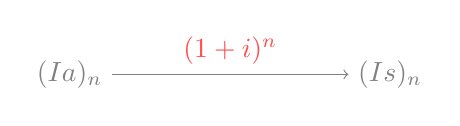
\begin{tikzpicture}
\draw [color=black!50,->](0,0) node[left]{$(Ia)_{\angles{n}}$}-- node [color=red!70,pos=0.5,above,sloped]{$(1+i)^n$}(3,0) node[right]{$(Is)_{\angles{n}}$};
    \end{tikzpicture} \\
\section{复递增年金}

$(Ca)_{\angles{n}}$:复递增年金
\begin{definition}{期末付复递增年金}
\noindent $(Ca)_{\angles{n}}=\frac{(a)_{\angles{n}}}{1+r}(r\neq i)(j=\frac{i-r}{1+r})$
\end{definition}
\begin{remark}
\noindent $(Ca)_{\angles{n}}=v+(1+r)v^2+(1+r)^2v^3+\dots+ (1+r)^{n-1}v^n$
\end{remark}

\section{每年支付m 次的递增年金}
$$(I a)_{\angles{n}}^{(m)}=\frac{i}{i^{(m)}}(I a)_{\angles{n}}=\frac{\ddot{a}_{\angles{n}}-n v^{n}}{i^{(m)}}$$
% Please add the following required packages to your document preamble:
% \usepackage{multirow}
% Please add the following required packages to your document preamble:
% \usepackage{multirow}
